\documentclass[journal=jprobs,manuscript=article]{achemso}

\usepackage[version=3]{mhchem} % Formula subscripts using \ce{}
\usepackage[T1]{fontenc}       % Use modern font encodings
\usepackage{multirow}
\usepackage{subcaption}
\usepackage{booktabs}
\usepackage{hyperref}

\newcommand*\mycommand[1]{\texttt{\emph{#1}}}

\author{Stefan K. Solntsev}
\email{solntsev@wisc.edu}
\author{Michael R. Shortreed}
\author{Brian L. Frey}
\author{Lloyd M. Smith}
\affiliation[UwMadison]
{University of Wisconsin-Madison}
	
\title[Rapid and Accurate Global PTM Discovery (G-PTM-D) Using Post-Acquisition Spectral Calibration and Defined Mass Windows]
  {Rapid and Accurate Global PTM Discovery (G-PTM-D) Using Post-Acquisition Spectral Calibration and Defined Mass Windows}

\begin{document}

\begin{abstract}

Correct identification of protein post-translational modifications (PTMs) is crucial to understanding many aspects of protein function in biological processes.
G-PTM-D\cite{Li_2016} is a recently developed tool for global identification and localization of PTMs.
Spectral file calibration prior to applying G-PTM-D, and algorithmic enhancements in the peptide database search shown here significantly increase the accuracy and speed of PTM identification.
We enhance G-PTM-D by using targeted mass-window searches, and demonstrate its effectiveness in identification of numerous types of PTMs, including high-mass modifications such as glycosylations.
The changes described in this work lead to a 20\% increase in the number of identified modifications and an order of magnitude decrease in the search time.
Targeted mass-window searches are also shown to be useful in contexts other than G-PTM-D, producing superior results when used instead of standard narrow-mass and wide-mass searches.
\end{abstract}

\section{Introduction}

Many peptide residue modification types are known, and databases containing detailed information about such modifications are readily available\cite{Creasy_2004}.
Information about a modification often includes the chemical or isotopic composition, mass, specificity to certain residues, and possible restriction of placement to peptide or protein termini.
Despite the extensive cataloging of the different possible protein modifications, their comprehensive discovery and identifications in complex biological samples has continued to pose a difficult challenge for proteomics\cite{Olsen_2013}.

Numerous procedures for identification and localization of PTMs from "bottom-up" tandem mass spectrometric datasets exist, and those concentrate on easily studied modifications (e.g. phosphorylations) in well studied systems.
Global discovery tools, such as MODa\cite{Na_2011} are available.
G-PTM-D\cite{Li_2016}, is one recently described bioinformatics tool for the discovery and localization of new PTMs in unenriched samples that enables high confidence identification and discovery of a wide variety of different PTMs at the same time.
The G-PTM-D workflow consists of three stages: 1) A wide-mass database search\cite{Chick_2015, Na_2011} that provides spectral matches to unmodified peptides along with the mass differences between the identified peptides and the measured parent peptide masses (hypothesized to differ in mass due to the presence of a PTM).
2) For those peptides for which the mass difference corresponds to the mass of a known PTM, a database augmentation step adds plausible localized PTMs to the proteins in the search database.
3) A final standard narrow-mass search of the augmented database to identify both modified and unmodified peptides subject to the standard FDR threshold (e.g. 1\% FDR).

As described, G-PTM-D has a few significant limitations.
The initial wide-mass search procedure is slow, taking hours for modest size datasets.
Due to this, high mass modifications, such as glycosolations are out of reach, since widening the search window from the suggested $\pm 200$ Daltons increases the search time even more.
Furthermore, in G-PTM-D, modification discovery is limited to PTMs in the Uniprot database. 
Finally, PTMs that are similar in mass, such as phosphorylation and sulfonation are problematic since they are virtually indistinguishable in unprocessed spectra files.
These three limitations motivated the work described here.

Spectral calibration is essential for distinguishing modifications with similar mass, so we recommend running the G-PTM-D procedure only on calibrated spectra files.
We present an enhancement to G-PTM-D, that addresses the long search times of the wide-mass search, and the limitations of the standard final narrow-mass search.
MSFragger, a method recently described in\cite{Kong_2017}, significantly decreases the runtime of wide-mass searches, but lacks specificity.
Thererfore, we replace the wide-mass search in the first stage by a specialized search that only allows specific mass differences which correspond to pre-selected modification masses.
This change improves the specificity and significantly decreases search time.
The final narrow-mass search is also replaced by a specialized missed-monoisotope identifying search, further increasing the number of confidently identified peptides. 

The idea of restricting the search space by only allowing certain mass differences between the precursor and the identified peptide mass is useful in other procedures as well, beyond the G-PTM-D workflow.
Its efficacy is demonstrated in context of a search for novel modifications, that is usually based on a wide-mass or an open-mass search.
A combination of specialized notch and interval searches produces superior identification and discovery results.

\begin{figure}[H]
  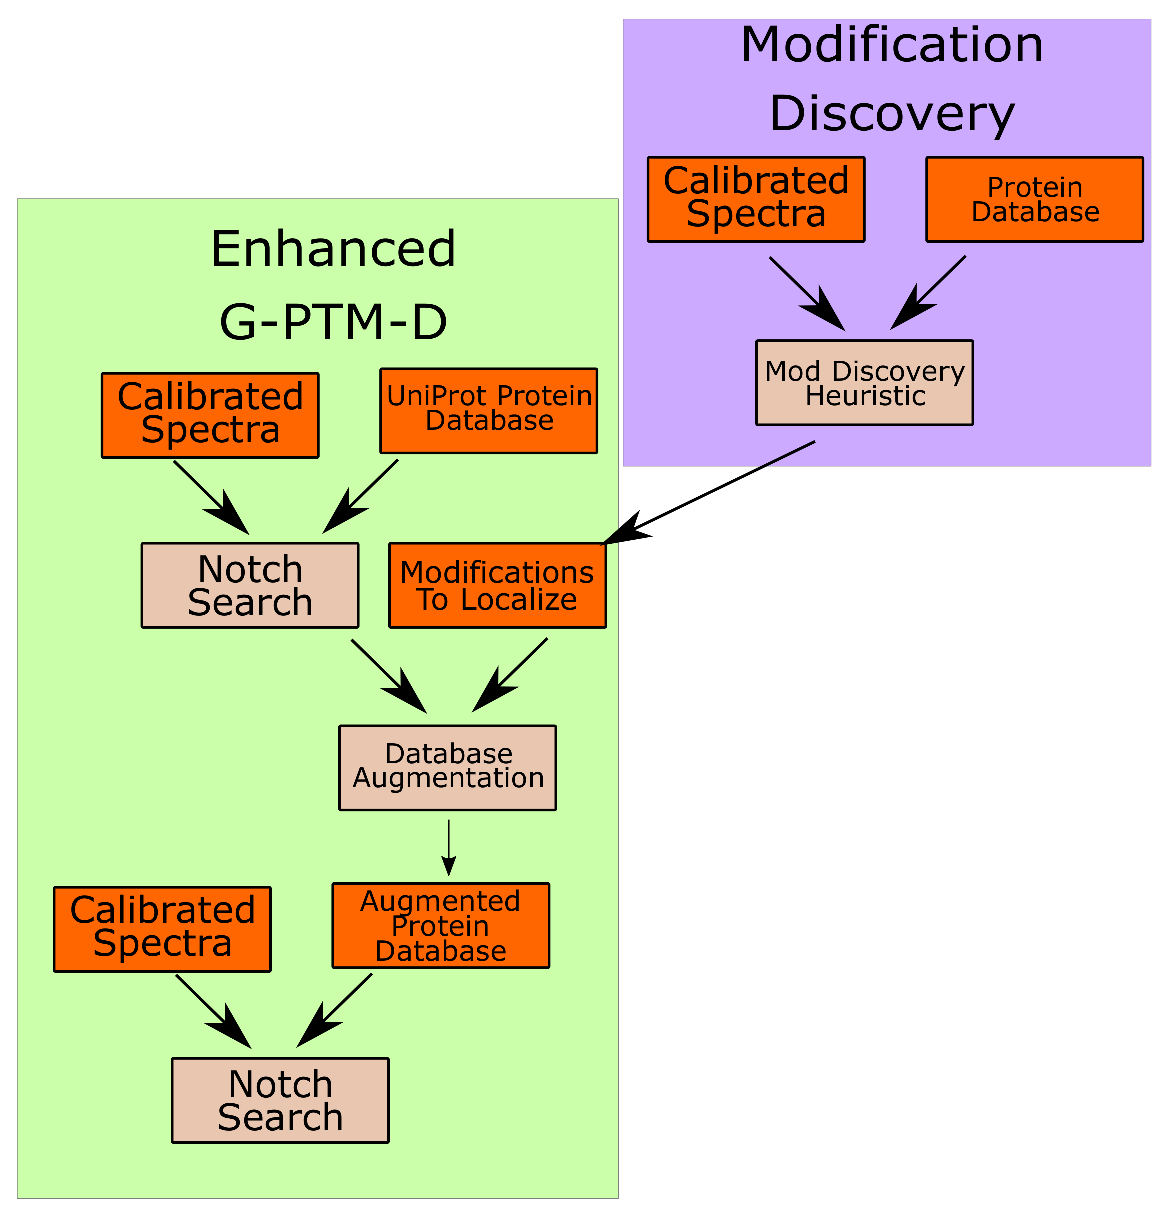
\includegraphics{diagram.eps}
  \caption{Workflows}
  \label{fgr:diagram}
\end{figure}


\section{Experimental Procedures}
We developed a modified version of the Morpheus software for bottom-up spectral database searching\cite{Wenger_2013} that we call MetaMorpheus\footnote{Free and Open Source software available at \url{https://github.com/smith-chem-wisc/MetaMorpheus}}, which integrates the database search procedure with spectral calibration and the G-PTM-D workflow.
Two multi-fraction mammalian datasets (\textit{Mouse} and \textit{Jurkat}) with deep proteome coverage were used to evaluate performance. These tryptically digested cell lysates correspond to 18 and 27 spectra files (fractions) respectively, and are described in detail in~\cite{Shortreed_2015, Cesnik_2016}.
Uniprot XML protein databases acquired on Feb 27, 2017 containing only reviewed human/mouse proteins were employed. 

A 10ppm precursor mass tolerance was used for the initial calibration step, and then reduced to 5ppm for subsequent notch searches.
For the database augmentation step, we allowed 120 modifications including PTMs, adducts, and chemical modifications.
Final notch search used notches centered at \{0, 1.0029, 2.0052, 3.0077\} in order to capture missed identifications due to missed monoisotopic peaks.

For the discovery of novel modifications, we used a combination of two searches: A notch search with notches at all combinations of up to 2 residue mass additions or removals, and an interval search with lower bound of -187 Daltons, and with exclusions at masses corresponding to the notch search.

\section{Results and Discussion}

This work recommends introducing two major changes to the standard G-PTM-D workflow: a spectral calibration, and a replacement of the standard searches with custom mass-window type searches.
In order to clearly show the advantage of each proposed change, they are initially discussed in isolation, and then the following section shows the combined effect on the overall PTM identification.

%The first modification to the G-PTM-D workflow, post-acquisition calibration, is shown to increase the number of confidently identified peptides, and enables qualitatively distinguishing modifications with similar mass.
%The other major enhancement, the mass-window search, is contrasted with the narrow-mass and open-mass search.
%The superior performance of G-PTM-D achieved by the use of mass-window searches is demonstrated.
%Finally, the application of mass-window searches to the discovery of novel modifications is discussed.

\subsection{Calibration}

A critical parameter for peptide identification is mass accuracy\cite{Scherl_2008}.
Higher mass accuracy provides increased specificity and thus confidence in peptide identifications, decreasing the false discovery rate.
Instrument noise, systemic drift and miscalibration limit the mass accuracy in acquired spectra.
Multiple calibration strategies to improve mass accuracy have been devised, and fall into three general categories:  External calibration prior to the MS experiment (e.g. standard instrument calibration protocols); internal calibration during the MS experiment (e.g. real-time calibration using a lock mass standard\cite{Olsen_2005}); and subsequent to the MS experiment (post-acquisition spectral calibration).
We use a post-acquisition calibration procedure that builds upon the software lock mass concept\cite{Cox_2011} recently reported by the Mann group.
In our strategy, the m/z differences between expected and observed peaks in the peptide tandem ms spectra are compiled, and then used to recalibrate the spectra.
%The increased mass accuracy of the calibrated spectra leads directly to improved identifications of both modified and unmodified peptides, as well as to increased confidence for PTM localization.

The spectral calibration procedure consists of two steps: Step 1: A narrow tolerance (e.g. 10 ppm precursor, 0.01 Dalton fragment) database search is performed on the dataset.
This yields a set of peptide identifications subject to a desired false discovery rate (e.g 1\%; based upon the target:decoy strategy \cite{Elias_2007}).
Step 2: The identifications from Step 1 are used to extract peak matches from the spectra, and a peak shifting procedure is performed.
The calibration algorithm is described in detail in Supplementary Material 1.

Calibration quality is accessed through the results of a standard 10ppm precursor tolerance database search.
PSMs within 1\% FDR prior to calibration are compared with PSMs after the calibration procedure, see Table~\ref{tbl:calib}.
The calibration procedure successfully addresses instrument miscalibration by centering the average error around zero.
Furthermore, the systemic noise introduced by various other factors is addressed: this is evident in the decrease in the standard deviation of the errors in the precursor mass estimates, which places calibrated data squarely in the sub-ppm mode.
Histograms of the mass errors before and after calibration are plotted in Figure~\ref{fgr:figure1}.

\begin{table}[]
\centering
\caption{PSMs Within 1\% FDR Before and After Calibration}
\label{tbl:calib}
\begin{tabular}{@{}llllll@{}}
                                                                                &        & \multicolumn{2}{l}{Mouse} & \multicolumn{2}{l}{Jurkat} \\ \cmidrule(l){3-6} 
                                                                                &        & Orig        & Calib       & Orig        & Calib        \\ \cmidrule(l){3-6} 
\multicolumn{2}{l}{PSM Count}                                                            &    152208       &        155617 &         217612   &   219172        \\
\multicolumn{2}{l}{Average Error (ppm)}                                                           &    -1.09         &       -0.16      &      -2.10      &        -0.16      \\
\multicolumn{2}{l}{St. Dev of Error}                                                     &     3.35        &      0.90       &       2.15      &        0.91      \\
\multirow{3}{*}{\begin{tabular}[c]{@{}l@{}}Confidence\\ Intervals\end{tabular}} & 68.3\% &   [-4.44,2.27]          &    [-1.06,0.74]          &    [-4.26,0.05]          &  [-1.08,0.75]            \\
                                                                                & 95.4\% &   [-7.80,5.62]          &    [-1.97,1.64]         &   [-6.41,2.20]          &      [-1.99,1.61]         \\
                                                                                & 99.7\% &   [-11.15,8.98]          &      [-2.87,2.54]        &    [-8.56,4.36]          &      [-2.90,2.58]         \\ \cmidrule(l){3-6} 
\end{tabular}
\end{table}

\begin{figure}
  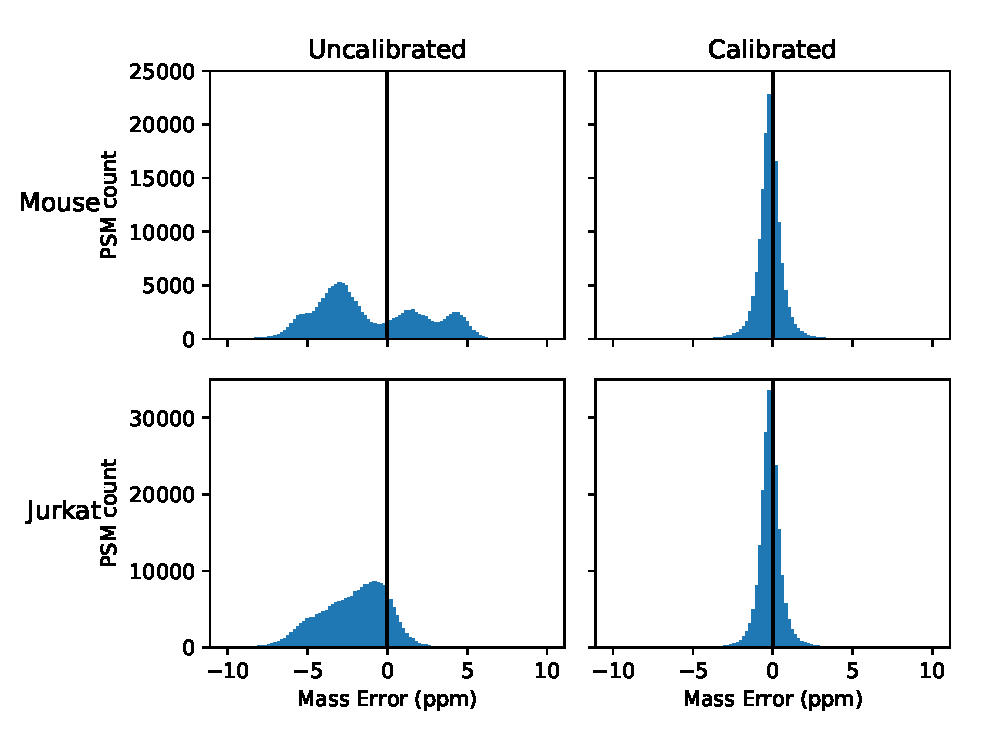
\includegraphics{fig2-calibrationQuality.eps}
  \caption{Histograms demonstrating the effect of calibration on PSM mass errors}
  \label{fgr:figure1}
\end{figure}

Besides simply increasing the number of confidently identified peptides, calibration is instrumental in increasing the discernibility between different mass shifts. A search that allows mass differences in the interval [79.942541, 79.980605] was conducted: the resultant mass shifts are aggregated in the histogram plots below. It is evident that the phosphorylation and sulfonation peaks are clearly separated and identifyable when the search is conducted on calibrated data.


\begin{figure}
  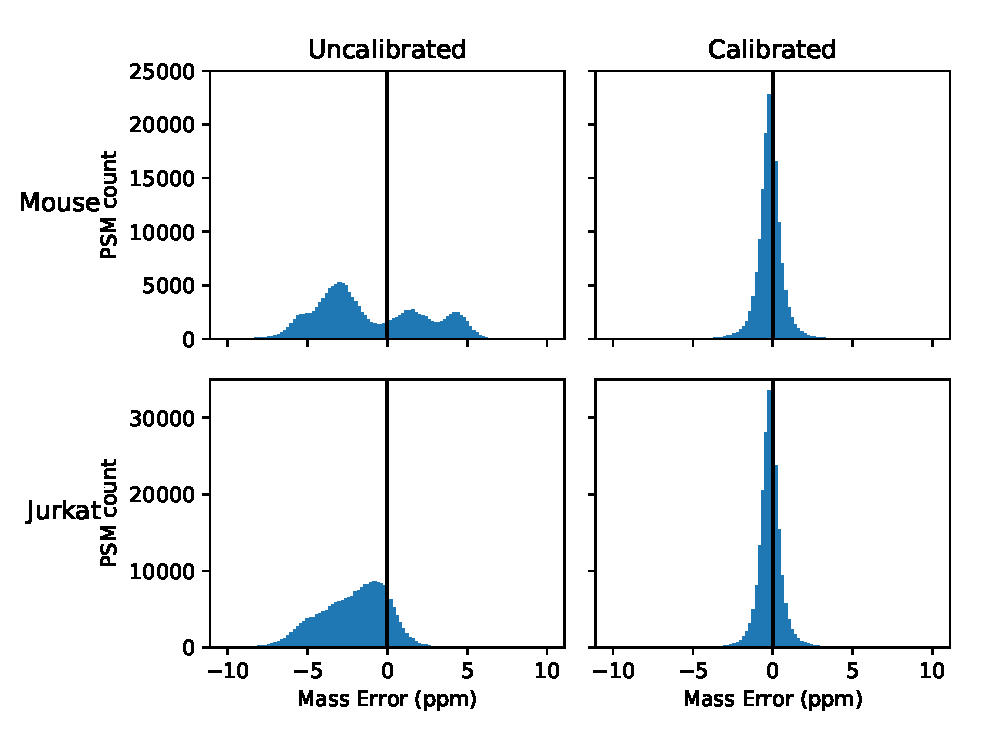
\includegraphics{fig2-calibrationQuality.eps}
  \caption{Histograms demonstrating the effect of calibration on PSM mass errors}
  \label{fgr:figure1}
\end{figure}
\newpage

\subsection{Mass-Window Searches}

Prior to discussing the impact mass-windows searches have on the G-PTM-D workflow, we need to define the search modes discussed. A standard \textit{narrow-mass} search considers matching theoretical peptides to spectra if the peptide mass and the identified precursor mass are equal, within some tolerance (i.e. 5ppm, or 2.1 Da).
A \textit{wide-mass} search matches peptide fragment masses to fragmentation spectra while allowing large differences (i.e. $\pm 500$ Da) between the observed precursor mass and the peptide mass.
An even less restrictive \textit{open-mass} search, matches peptides from a database to fragmentation spectra without taking the precursor mass into account.
We describe alternatives to these search modes, namely a \textit{notch search} and an \textit{interval search} that fall under a broad category of \textit{mass-window} searches.
The notch search is an extension of the narrow-mass search: it allows exact matches (within a tolerance) to specific mass differences between the theoretical peptide and observed precursor masses.
The interval search is an extension of the wide-mass search: specific problematic mass differences are excluded from allowed matches.
Figure~\ref{fgr:differentSearchModes} provides a convenient way to visualize the various search modes.

\begin{figure}
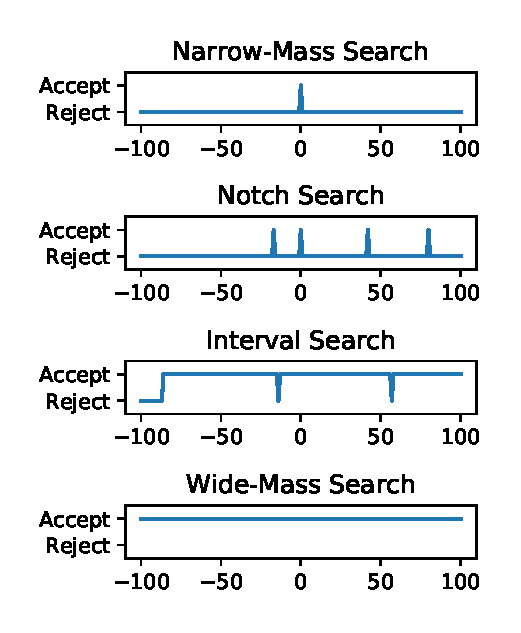
\includegraphics{fig1-searchTypes.eps}
\caption{Search Modes}
\label{fig:fig1-searchtypes}
\end{figure}

\subsubsection{Notch Search vs Narrow-Mass Search}

The purpose of a narrow-mass search is to use the provided precursor mass along with fragmentation spectra information to find an exact match to the observed peptide in a protein database.

Using a calibration or instrument noise percursor tolerance, such as 5ppm or 10ppm is a valid approach, since it identifies only exact matches.
A major drawback of this strategy is that it misses monoisotope errors.
To avoid this complication, and to get a more comprehensive list of matches, a wider search tolerance is often used, e.g. $\pm 3.5$ Da.
This gives a substantially larger list of matches, and the resulting PSMs with non-zero mass shifts could be attributed to missed monoisotopes or co-isolated peptides.
While this approach provides a larger list of confident PSMs, a substantial fraction of those is wrong, since certain mass shifts in the chosen Dalton range arise due to sequence variations or PTMs.
These require an extensive framework (such as G-PTM-D) to identify and label them.
More importantly, those modified peptides \textit{do not} correspond to the identified one, thus arguably defeating the purpose of a narrow-mass search. 

We observe that when using an incomplete database that does not include comprehensive modification and sequence variation information, a notch search with notches at monoisotopic peaks is superior to either of the narrow-mass searches.

\begin{table}[]
\centering
\caption{Notch Search vs Narrow-Mass Search comparison of PSMs for Mouse}
\label{my-label}
\begin{tabular}{@{}llll@{}}
                    & 5ppm Search & 3.5 Da Search & Notch Search \\ \cmidrule(l){2-4}
PSMs Within 1\% FDR & 157188      & 178003        &        \\
MisAssigned PSMs    & 0           &               & 0            \\
Good PSMs           & 157188      &         &        \\ 
\end{tabular}
\end{table}

\begin{figure}
\caption{Mouse histograms around 0}
\label{fig:fig3mouse-1012}
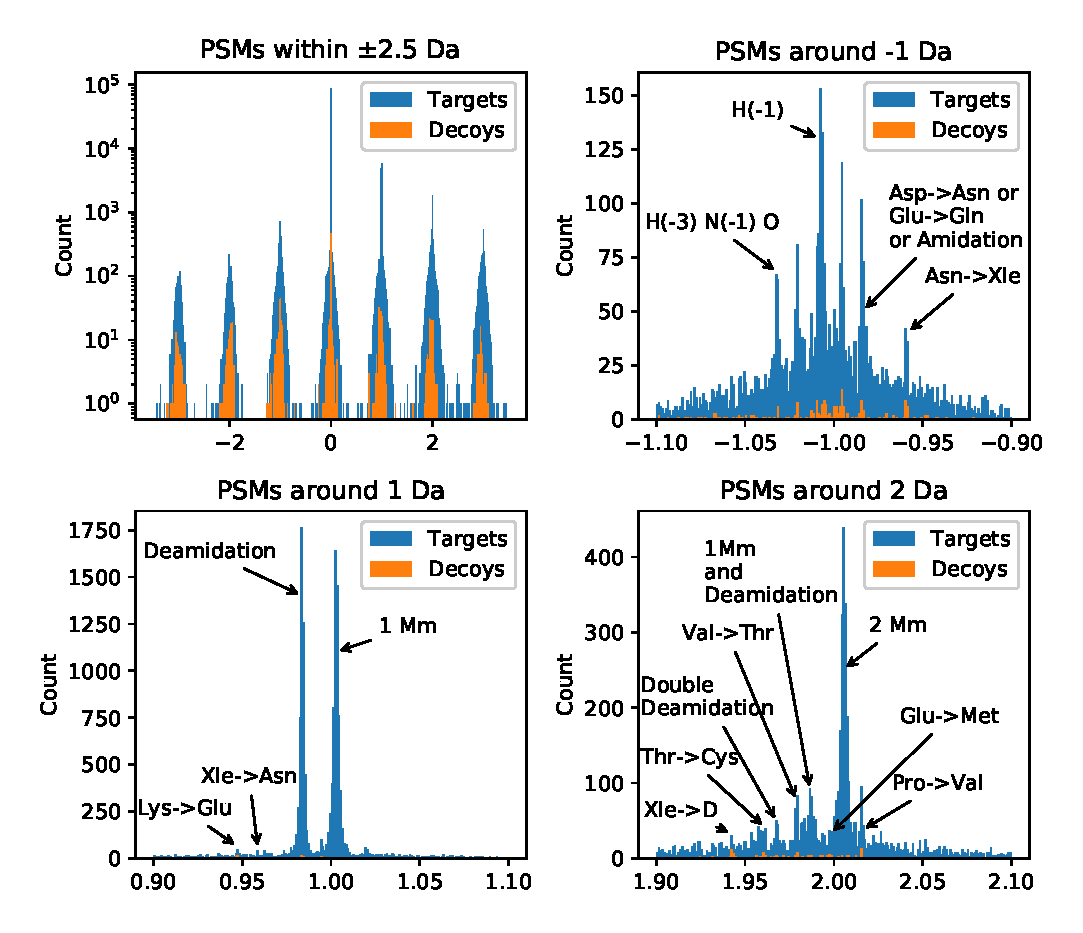
\includegraphics{fig3mouse-1012}
\end{figure}

\begin{figure}
\caption{Jurkat histograms around 0}
\label{fig:fig3jurkat-1012}
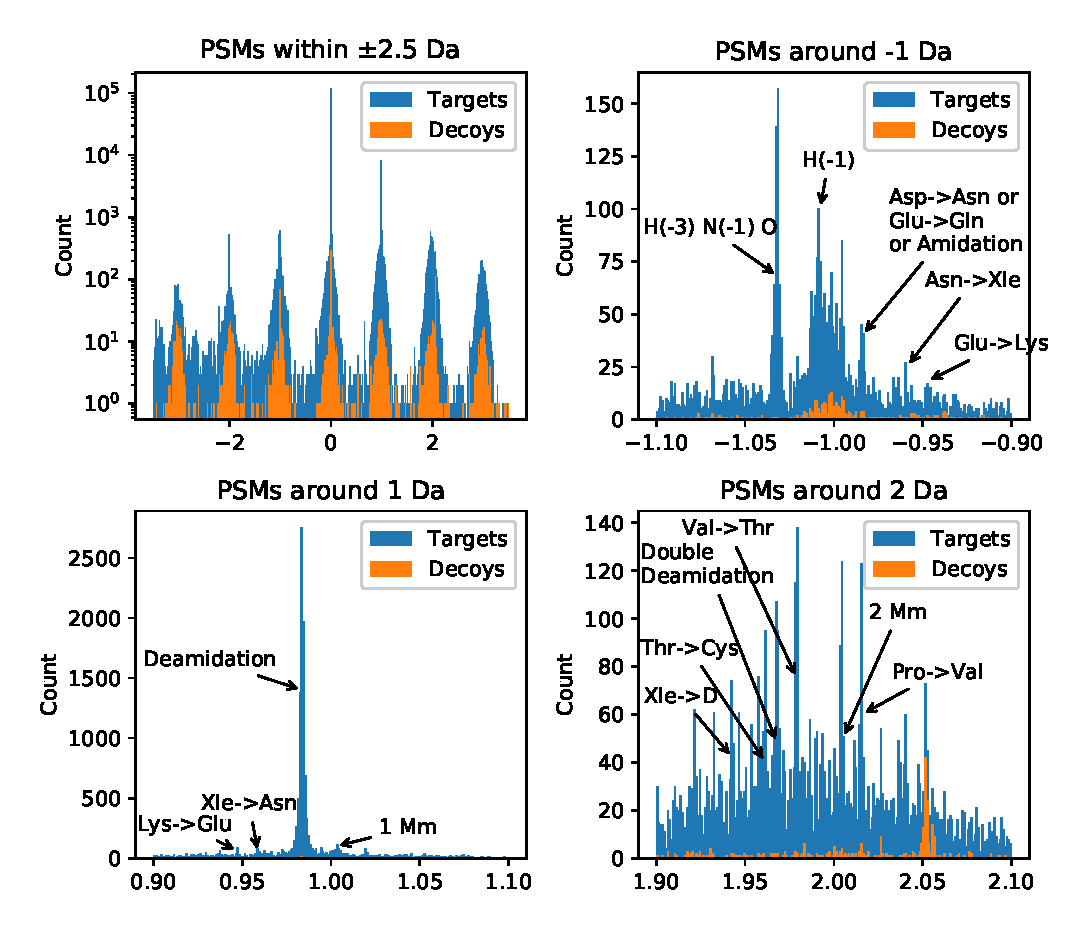
\includegraphics{fig3jurkat-1012}
\end{figure}



\subsubsection{Mass-Window Searches vs Open-Mass Search}

Restricting the allowed precursor masses is beneficial in searches that are intended to discover mass shift peaks.
We ran a completely open precursor mass search, and restricted ourselves to looking at 1\% FDR matches, both targets and decoys.
The plots in Figure~\ref{fig:figure2-upperlowerbounds} show the FDR in the list filtered by using a lower or upper bound cutoff on the allowed mass shifts.
It shows the fundamental difference between upper and lower bound cutoffs: while it is beneficial to restrict open searches to ignore large negative values, restricting matches with a large positive mass difference has a negative effect on the overall FDR.

This effect can be explained by the fact that it's easier to match long sequences to short peptide fragmentation profiles than it is to match short sequences to fragmentation pattern of a long peptide.

\begin{figure}
\caption{Upper and Lower bound cutoffs in Mouse Data}
\label{fig:fig4-limitsOnOpenSearch}
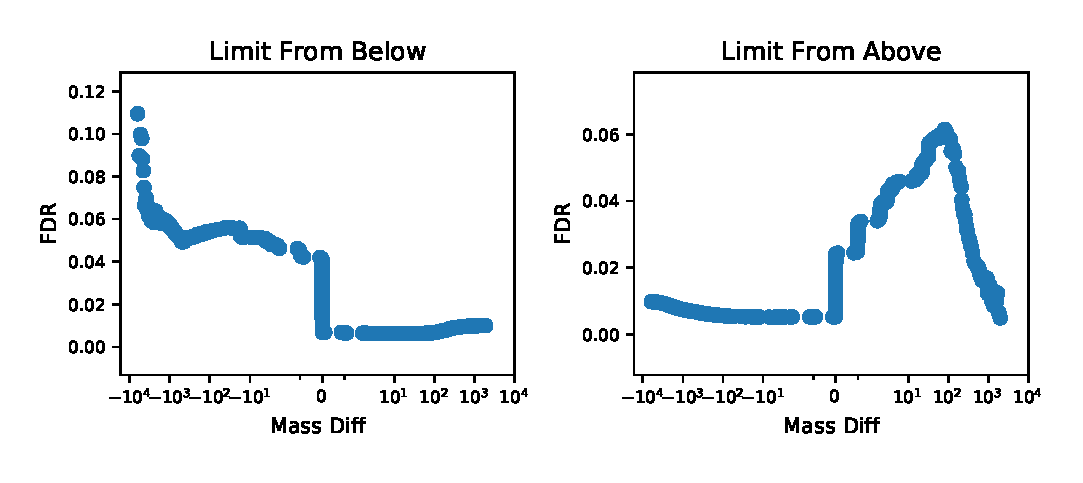
\includegraphics{fig4-limitsOnOpenSearch}
\end{figure}

MetaMorpheus includes a capability to identify peaks in a mass shift histogram obtained from a search, using a recently described peak finding algorithm\cite{Rodriguez_2014}.
We identified peaks with anomalously high false discovery rates, which could be excluded from wide mass searches in order to improve the overall identification quality.
Some histogram peaks are illustrated in Figure~\ref{fig:figure3}, including peaks corresponding to masses of Sulfo and Phospho, and a problematic peak at mass of Leucine, with a high FDR.

\begin{figure}
\caption{Some Histogram Peaks For Mouse Data}
\label{fig:fig5-HistogramsAround80and113}
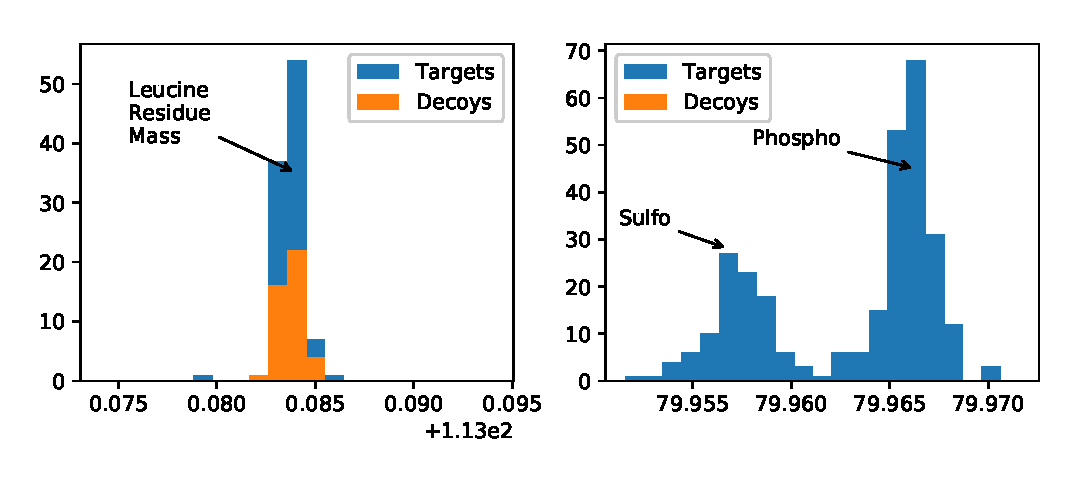
\includegraphics{fig5-HistogramsAround80and113}
\end{figure}

We identified the property of some specific mass shifts that correspond to anomalously high false discovery rates: these mass shifts correspond precisely to various combinations of residue mass additions and removals.

Mass windows provide an mechanism to exclude these problematic mass shifts from a wide-mass search by employing a interval search.

\subsection{G-PTM-D}

By employing the novel notch search strategy instead of the wide-mass search in the G-PTM-D process, using only the modifications listed in Uniprot, the number of confidently identified PSMs increased by 6\%.
The overall search time dropped significantly, from 35 hours to 4 hours for all datasets, see Table~\ref{my-label}.

\begin{table}[]
\centering
\caption{Effects of Replacing Initial Wide-Mass Search by a Notch Search}
\label{my-label}
\begin{tabular}{ll|l|l}
                      &        & Wide-Mass Search & Notch Search\\
\hline
\multirow{2}{*}{Time} & Jurkat & 22.1 hrs         & 2.9 hrs    \\
                      & Mouse  & 13.5 hrs         & 1.2 hrs   \\
\hline
\multirow{2}{*}{PSMs} & Jurkat & 203237           & 210566    \\
                      & Mouse  & 153674           & 162473   
\end{tabular}
\end{table}


The final search with the augmented database is conducted with notches: we only recommend including the common missed monoisotopic mass values in the final search,.
The effect of using these notches is shown in Table~\ref{tab:table2}.

\begin{table}[]
\centering
\caption{Effects of Replacing Final Narrow-Mass Search by a Notch Search}
\label{tab:table2}
\begin{tabular}{ll|l|l}
                      &        & Narrow-Mass Search & Notch Search\\
\hline
\multirow{2}{*}{PSMs} & Jurkat  & 210566   &  220574  \\
                      & Mouse    & 162473   &   170743
\end{tabular}
\end{table}

Since the XML database is annotated with PTMs from the UniProt PTM list, it is natural to use it in the augmentation step as well.
It has a few significant drawbacks: Some mass values do not correspond to actual mass shifts, lability of modifications is not taken into account, and many PTMs are missing, including adducts and glycosylations.
Notch searches allow using expanded modification lists that include chemical modifications such as adducts and large mass PTMs such as glycosylations.
Even though adducts arising from experimental artifacts are not ultimately interesting to biologists, not including them as an option decreases the total number of identified proteins and PTMS.
A curated set of notches and the corresponding modifications is given in Appendix A.
The overall identification rate increased from 164,697 to 179,345 peptide-spectral matches (PSMs), which in turn increased the number of modified peptides by an additional 20\%.
We identified hundreds of glycosylated peptides in these unenriched samples, with many of these modifications exceeding 1000 Daltons. 

\begin{table}[]
\centering
\caption{Effects of Using Different Modification Lists}
\label{tab:table3}
\begin{tabular}{ll|l|l|l}
                      &        & Only Uniprot & Uniprot+Glyco & Uniprot+Glyco+Adducts\\
\hline
\multirow{2}{*}{PSMs} & Jurkat  & 220574   &  222985 & 223578\\
                      & Mouse    & 170743   &   171432& 174783 
\end{tabular}
\end{table}

The initial notch search is significantly faster than a corresponding wide mass search, and this suggests that multiple search rounds could be conducted, iteratively adding more and more modifications.
This recursive nature of the algorithm is well suited to add multiple modifications of different types on the same peptide.
Due to these enhancements, we test the performance of our methods 

\begin{table}[]
\centering
\caption{My caption}
\label{my-label}
\begin{tabular}{|l|l|l|l|l|l|}
\hline
                      &        & \multicolumn{2}{l|}{Single Round}                                                                              & \multicolumn{2}{l|}{Multiple Rounds}                                                                           \\ \hline
                      &        & \begin{tabular}[c]{@{}l@{}}Mods:\\ none\end{tabular} & \begin{tabular}[c]{@{}l@{}}Mods:\\ ptmlist\end{tabular} & \begin{tabular}[c]{@{}l@{}}Mods:\\ none\end{tabular} & \begin{tabular}[c]{@{}l@{}}Mods:\\ ptmlist\end{tabular} \\ \hline
\multirow{2}{*}{PSMs} & Jurkat &                                                      &                                                         &                                                      &                                                         \\ \cline{2-6} 
                      & Mouse  &                                                      &                                                         &                                                      &                                                         \\ \hline
\multirow{2}{*}{Mods} & Jurkat &                                                      &                                                         &                                                      &                                                         \\ \cline{2-6} 
                      & Mouse  &                                                      &                                                         &                                                      &                                                         \\ \hline
\multirow{2}{*}{Time} & Jurkat &                                                      &                                                         &                                                      &                                                         \\ \cline{2-6} 
                      & Mouse  &                                                      &                                                         &                                                      &                                                         \\ \hline
\end{tabular}
\end{table}


\subsection{Discovery of Modifications not in Database}

Previously described wide mass search strategies for discovery and localization of unknown modifications benefit from using alternative, carefully designed search modes based on interval and notch searches.
We discovered that limiting mass shifts to a lower bound of -187 Da (corresponding to the largest mass difference that could be attributed to loss of a single residue, Tryptophan), and no upper bound, is an important step in eliminating spurious PSMs.
Furthermore, treating highly suspect mass shifts corresponding to residue additions/substitutions/deletions in a separate notch search with individualized false discovery rate estimates is beneficial.
An automated tool built into MetaMorpheus allows confidently identifying novel modifications based on these search results.


%
\begin{acknowledgement}

The authors thank \ldots
\end{acknowledgement}

\begin{suppinfo}

The following files are available free of charge.
\begin{itemize}
  \item Filename: brief description
  \item Filename: brief description
\end{itemize}

\end{suppinfo}

\newpage

\bibliography{citations}

\end{document}
